% Options for packages loaded elsewhere
\PassOptionsToPackage{unicode}{hyperref}
\PassOptionsToPackage{hyphens}{url}
%
\documentclass[
]{article}
\usepackage{amsmath,amssymb}
\usepackage{iftex}
\ifPDFTeX
  \usepackage[T1]{fontenc}
  \usepackage[utf8]{inputenc}
  \usepackage{textcomp} % provide euro and other symbols
\else % if luatex or xetex
  \usepackage{unicode-math} % this also loads fontspec
  \defaultfontfeatures{Scale=MatchLowercase}
  \defaultfontfeatures[\rmfamily]{Ligatures=TeX,Scale=1}
\fi
\usepackage{lmodern}
\ifPDFTeX\else
  % xetex/luatex font selection
\fi
% Use upquote if available, for straight quotes in verbatim environments
\IfFileExists{upquote.sty}{\usepackage{upquote}}{}
\IfFileExists{microtype.sty}{% use microtype if available
  \usepackage[]{microtype}
  \UseMicrotypeSet[protrusion]{basicmath} % disable protrusion for tt fonts
}{}
\makeatletter
\@ifundefined{KOMAClassName}{% if non-KOMA class
  \IfFileExists{parskip.sty}{%
    \usepackage{parskip}
  }{% else
    \setlength{\parindent}{0pt}
    \setlength{\parskip}{6pt plus 2pt minus 1pt}}
}{% if KOMA class
  \KOMAoptions{parskip=half}}
\makeatother
\usepackage{xcolor}
\usepackage[margin=1in]{geometry}
\usepackage{graphicx}
\makeatletter
\def\maxwidth{\ifdim\Gin@nat@width>\linewidth\linewidth\else\Gin@nat@width\fi}
\def\maxheight{\ifdim\Gin@nat@height>\textheight\textheight\else\Gin@nat@height\fi}
\makeatother
% Scale images if necessary, so that they will not overflow the page
% margins by default, and it is still possible to overwrite the defaults
% using explicit options in \includegraphics[width, height, ...]{}
\setkeys{Gin}{width=\maxwidth,height=\maxheight,keepaspectratio}
% Set default figure placement to htbp
\makeatletter
\def\fps@figure{htbp}
\makeatother
\setlength{\emergencystretch}{3em} % prevent overfull lines
\providecommand{\tightlist}{%
  \setlength{\itemsep}{0pt}\setlength{\parskip}{0pt}}
\setcounter{secnumdepth}{-\maxdimen} % remove section numbering
\usepackage{booktabs}
\usepackage{longtable}
\usepackage{array}
\usepackage{multirow}
\usepackage{wrapfig}
\usepackage{float}
\usepackage{colortbl}
\usepackage{pdflscape}
\usepackage{tabu}
\usepackage{threeparttable}
\usepackage{threeparttablex}
\usepackage[normalem]{ulem}
\usepackage{makecell}
\usepackage{xcolor}
\ifLuaTeX
  \usepackage{selnolig}  % disable illegal ligatures
\fi
\usepackage{bookmark}
\IfFileExists{xurl.sty}{\usepackage{xurl}}{} % add URL line breaks if available
\urlstyle{same}
\hypersetup{
  pdftitle={Proportion\_analysis},
  pdfauthor={Miaobing},
  hidelinks,
  pdfcreator={LaTeX via pandoc}}

\title{Proportion\_analysis}
\author{Miaobing}
\date{2024-08-06}

\begin{document}
\maketitle

\begin{verbatim}
## # A tibble: 1 x 3
##     age gender referendum
##   <int>  <int>      <int>
## 1    12     18         85
\end{verbatim}

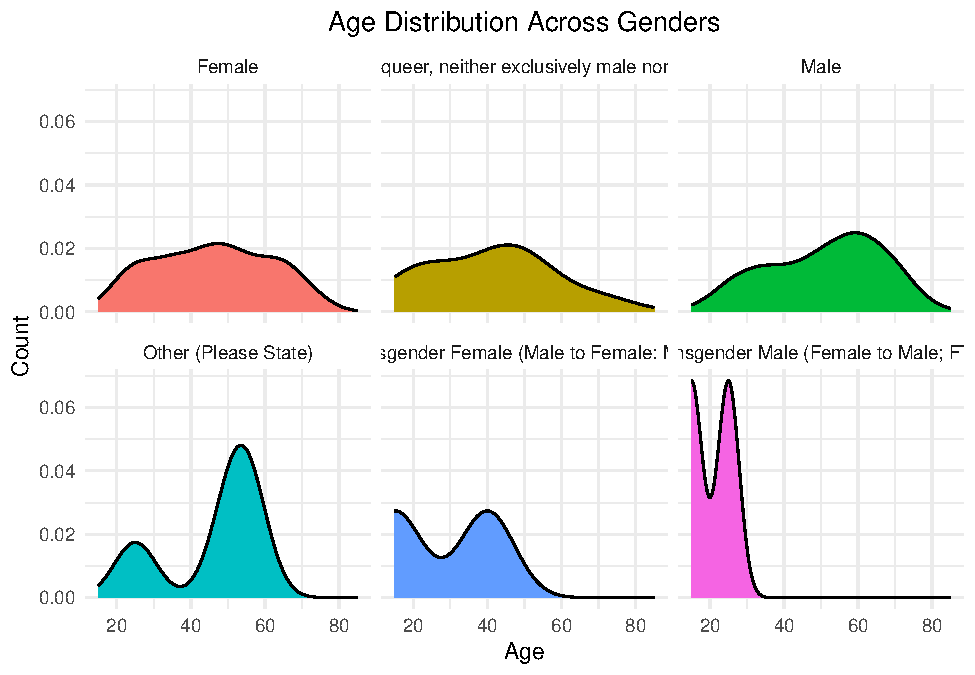
\includegraphics{Proportion_analysis_files/figure-latex/unnamed-chunk-4-1.pdf}
\# Complete cases \#\#\# 1. The proportion for vote `yes' in the
referendum

\begin{verbatim}
## [1] 0.6
\end{verbatim}

\subsubsection{2. Logistic regression table for Complete
cases}\label{logistic-regression-table-for-complete-cases}

\begin{longtable}[t]{lrrrr}
\caption{\label{tab:unnamed-chunk-6}Logistic Regression on Complete Cases}\\
\toprule
term & estimate & std.error & statistic & p.value\\
\midrule
(Intercept) & 1.9911196 & 0.2418370 & 8.2333136 & 0.0000000\\
age & -0.0291008 & 0.0045787 & -6.3557526 & 0.0000000\\
genderGenderqueer, neither exclusively male nor female & 1.3495750 & 1.0764310 & 1.2537496 & 0.2099330\\
genderMale & -0.4127509 & 0.1377062 & -2.9973304 & 0.0027236\\
genderOther (Please State) & 0.2548679 & 1.2291860 & 0.2073469 & 0.8357389\\
\addlinespace
genderTransgender Female (Male to Female: MTF) & 13.3899203 & 608.7668192 & 0.0219952 & 0.9824518\\
genderTransgender Male (Female to Male; FTM) & 13.1592764 & 621.6285024 & 0.0211690 & 0.9831108\\
\bottomrule
\end{longtable}

\section{Imputed cases}\label{imputed-cases}

\subsubsection{1. The proportion of yes
voters}\label{the-proportion-of-yes-voters}

\begin{verbatim}
## [1] 0.6
\end{verbatim}

\subsubsection{2. Logistic Regression Table for multiple
imputation}\label{logistic-regression-table-for-multiple-imputation}

\begin{longtable}[t]{lrrrrr}
\caption{\label{tab:unnamed-chunk-9}Logistic Regression on Imputed Data}\\
\toprule
term & estimate & std.error & statistic & df & p.value\\
\midrule
(Intercept) & 1.9907956 & 0.2615553 & 7.6113766 & 59.81544 & 0.0000000\\
age & -0.0293965 & 0.0048799 & -6.0239461 & 82.77097 & 0.0000000\\
genderGenderqueer, neither exclusively male nor female & 1.3638259 & 1.0773457 & 1.2659131 & 1032.92575 & 0.2058297\\
genderMale & -0.3960150 & 0.1371885 & -2.8866495 & 435.38010 & 0.0040875\\
genderOther (Please State) & 0.5014826 & 1.1705221 & 0.4284264 & 1033.82042 & 0.6684299\\
\addlinespace
genderTransgender Female (Male to Female: MTF) & 13.3989723 & 608.4891979 & 0.0220201 & 1035.89948 & 0.9824362\\
genderTransgender Male (Female to Male; FTM) & 13.1656106 & 621.5790396 & 0.0211809 & 1035.89948 & 0.9831054\\
\bottomrule
\end{longtable}

\section{Conclusion:}\label{conclusion}

Based on the analysis, the proportion of people in the sample who
supported legalisation is 0.59 using complete cases and 0.6 using
imputed data. The logistic regression interpret the results from the
logistic regression output.

\section{Comparison of Regression
Analyses}\label{comparison-of-regression-analyses}

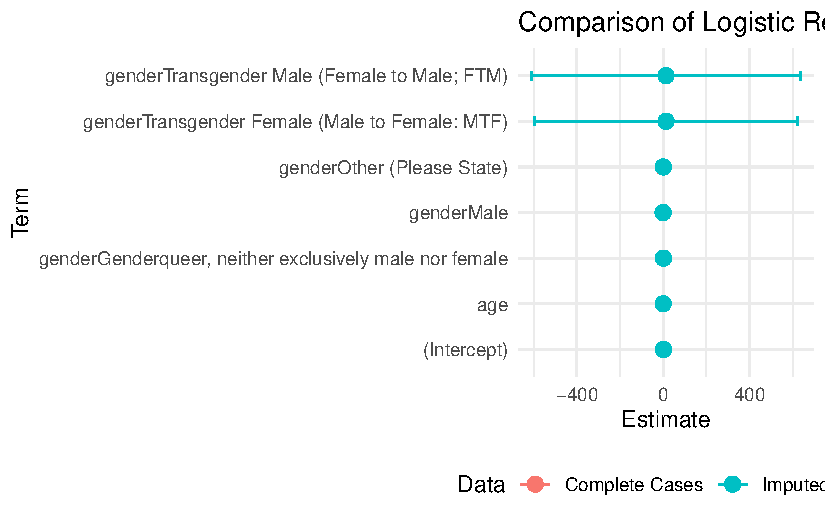
\includegraphics{Proportion_analysis_files/figure-latex/unnamed-chunk-10-1.pdf}

\end{document}
